%\documentclass[12pt,a4paper]{article}

\documentclass[hidelinks,11pt,twocolumn]{article}
\setlength{\columnsep}{35pt}

\renewcommand{\thesubsubsection}{\thesubsection.\alph{subsubsection}}

\usepackage[brazil]{babel}
\usepackage[utf8]{inputenc}
\usepackage[T1]{fontenc}
\usepackage{amsmath}
\usepackage{amsfonts}
\usepackage{makeidx}
\usepackage{amssymb}
\usepackage{graphicx}
\usepackage{helvet}
\usepackage{CJKutf8}
\usepackage[left=2cm,right=2cm,top=2cm,bottom=2cm]{geometry}
\usepackage{float}
\usepackage{hyperref}
%\usepackage[options]{natbib}


\begin{document}


\twocolumn[{%

	\begin{figure}[H]
%\centering
%\includegraphics[width = \linewidth]{fig\P2_M2.png}
\graphicspath{{Imagens/}}

\includegraphics[width = 0.5\linewidth]{UTFPR_jpeg.jpg}
\setlength{\abovecaptionskip}{0pt}
\setlength{\belowcaptionskip}{0pt}
%\caption{Synoptique du circuit}
\end{figure}

 \centering
 \LARGE \textbf{Projeto de uma Rede Neural Artificial \break para Reconhecimento Facial}
 
\ 
 
 \large \textbf{Matheus Augusto Wisniewski}
 
 Professora: Lucia Valeria Ramos de Arruda
 
 Disciplina: RNA - Redes Neurais Artificiais
 
 \textit{Universidade Tecnológica Federal do Paraná}
 
 \textit{Curitiba, Março de 2016}
	 
	 
	 \
	 
	 \
	 
	 \
 
}]

\textbf{Resumo:} Neste trabalho são apresentados os passos para a implementação de uma Rede Neural para o Reconhecimento Facial simples, além da justificativa da escolha de cada um deles.

\

\textbf{Palavras-chave:} Redes Neurais, Reconhecimento Facial

\section{Introdução}

O reconhecimento facial é uma tarefa tão comum aos seres humanos que um indivíduo nem percebe o inacreditável número de vezes que é realizado todos os dias, como ilustrado na Figura~\ref{diaadia}. 

Embora a pesquisa em reconhecimento facial automático venha sendo realizada desde a década de 1960, este tema capturou a atenção da comunidade científica apenas perto do ano 2000. Muitas técnicas de análise e modelagem de rosto têm progredido significativamente desde essa data \cite{fagertun}.

\begin{figure}[H]
\centering
%\includegraphics[width = \linewidth]{fig\P2_M2.png}
\graphicspath{{IMAGENS/}}
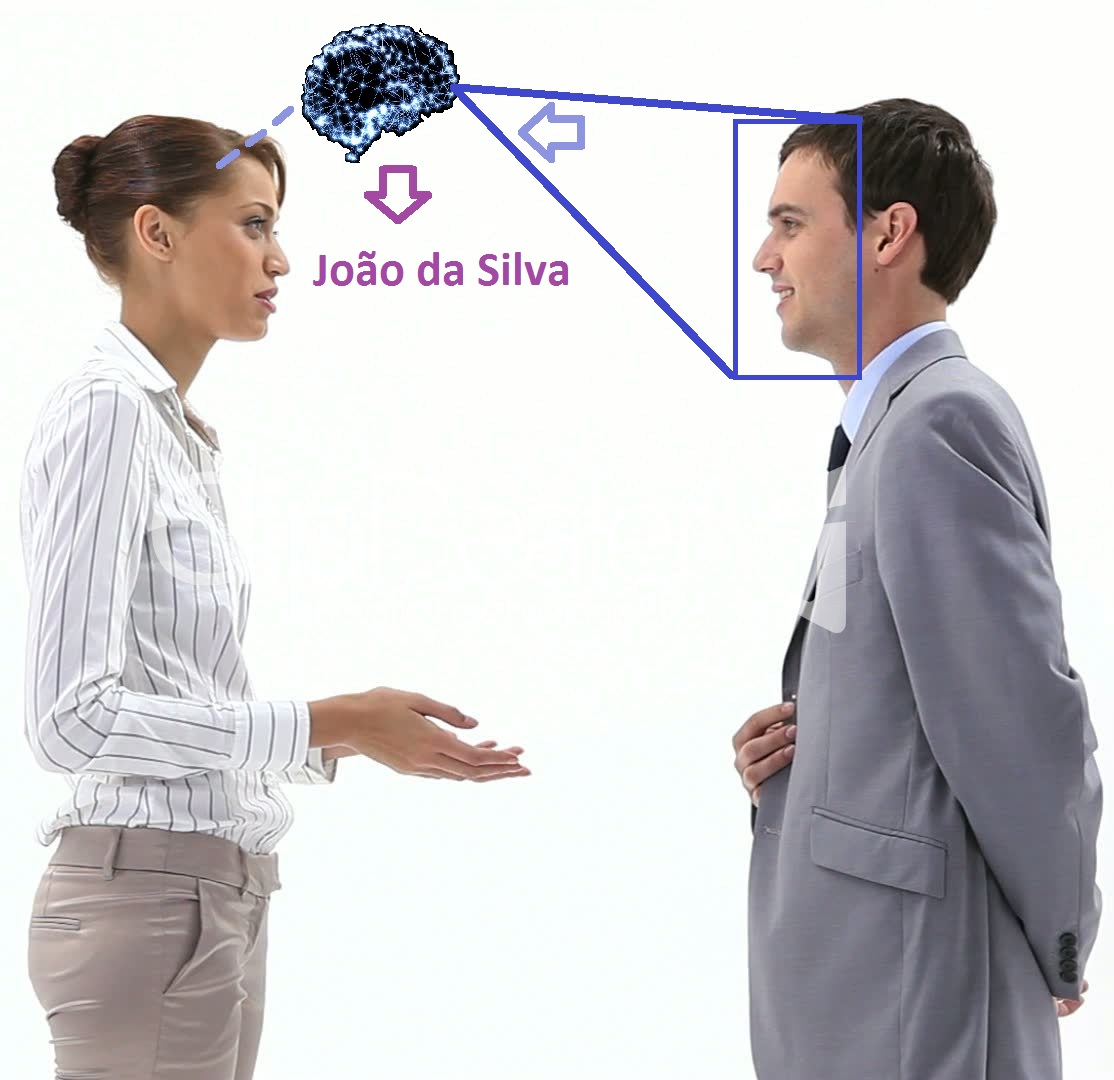
\includegraphics[width = 0.55\linewidth]{reconhecimento.jpg}
\setlength{\abovecaptionskip}{0pt}
\setlength{\belowcaptionskip}{0pt}
\caption{Reconhecimento facial no dia a dia}
\label{diaadia}
\end{figure}

\section{Objetivo}

O reconhecimento facial é um método não intrusivo, e imagens de rosto são a característica biométrica mais comumente utilizadas para reconhecimento de identidade \cite{yesu}. 

Além disso, a habilidade de realizar análise automática e confiável de rostos possibilita um número muito grande de aplicações. Existem utilidades na área de telecomunicações visuais (como a codificação e a melhoria da qualidade das imagens) e na área de segurança e monitoramento (como a interpretação mais inteligente das cenas), para citar algumas \cite{nightingale}.

Esses fatores somados ao objetivo de tornar o reconhecimento facial por redes neurais mais simples de ser entendido são as motivações principais desse trabalho.

\section{Justificativa}

A complexidade dos problemas de visão computacional é agravada pelo fato de que lida-se com enormes blocos de dados. A imagem em escala de cinza típica tem 640x480 pixels, cada um com 8-bits (ou 256 valores de cinza) de intensidade. Portanto, o tamanho de toda a imagem é 640x480x8 o que resulta no total de 2.457.600 bits \cite{balasuriya}. 

Por conta da altíssima quantidade de dados a serem processados, algoritmos de elevada complexidade tornam-se computacionalmente lentos e, consequentemente, deve-se optar por técnicas que simplifiquem o processamento \cite{balasuriya}.

Como se trata de um problema de reconhecimento de padrões, o reconhecimento facial consiste de três partes (após a detecção do rosto, como pode ser visto na Figura~\ref{blocos}): o alinhamento, a extração de características e a correspondência com o banco de dados. Essas últimas podem ser realizadas com alto desempenho através das redes neurais \cite{le}.

Este trabalho visa elucidar as fases posteriores à detecção de rostos, através de redes neurais.

\begin{figure}[H]
\centering
%\includegraphics[width = \linewidth]{fig\P2_M2.png}
\graphicspath{{IMAGENS/}}
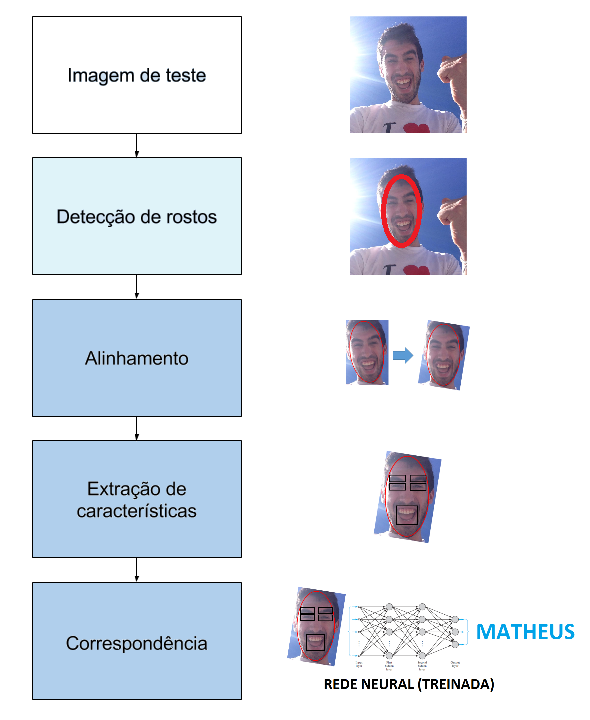
\includegraphics[width = 1\linewidth]{sistema.png}
\setlength{\abovecaptionskip}{0pt}
\setlength{\belowcaptionskip}{0pt}
\caption{Sistema de reconhecimento facial}
\label{blocos}
\end{figure}



\section{Descrição do problema}

O problema a ser tratado neste trabalho é o reconhecimento facial simples e replicável através de redes neurais.

\subsection{Localização do rosto}

A primeira etapa da Figura~\ref{blocos} foge do escopo deste estudo, já que para fins de teste pode-se utilizar uma base de dados e imagens de teste com a localização do rosto controlada, como a base de dados de rostos de Yale \cite{yale}, por exemplo. 

Alternativamente, algoritmos populares como o de Viola \& Jones \cite{viola-jones} também são recomendados para ambientes não-controlados.

\subsection{Identificação do rosto}

As três etapas que seguem a detecção do rosto na Figura~\ref{blocos} são de responsabilidade das redes neurais implementadas conforme descrito na \autoref{sect:construcao}.

\section{Construção do sistema neural}
\label{sect:construcao}

A escolha da rede neural foi baseada em um artigo que comparou a eficiência de várias combinações de redes neurais para o reconhecimento facial \cite{oravec}.


\subsection{Tipo de Rede}

A rede neural foi escolhida com base no estudo comparativo de eficiência de redes neurais feito por Oravec \& Pavlovicova \cite{oravec}, como pode ser visto na Tabela~\ref{tab:redes}:

\begin{table}[H]
\centering

\begin{tabular}{|c|c|}
\hline
\textbf{Redes Neurais} 	& \textbf{\% de sucesso} \\ \hline
PCA-hlo{MLP} 				& 83,07 \\ \hline
blockMLP-RBF 				& 82,29 \\ \hline
PCA 								& 81,51 \\ \hline
blockSOM-RBF				& 80,73 \\ \hline
blockSOM-MLP				& 79,95 \\ \hline
RBF								& 78,12 \\ \hline
MLP								& 78,12 \\ \hline
MLP-MLP						& 74,74 \\ \hline
blockMLP-MLP				& 73,70 \\ \hline
MLP-RBF						& 72,40 \\ \hline
\end{tabular}
\caption{Comparativo de redes neurais \cite{oravec}}
\label{tab:redes}
\end{table}

Pela facilidade de implementação, aliada com a grande eficiência, a rede neural escolhida foi a \textbf{blockMLP-RBF}.

Esta é a combinação de uma rede Perceptron Multicamadas (MLP, do inglês \textit{Multi-Layer Perceptron}) no início, para comprimir a imagem inicial (extraindo dessa forma as características principais), e uma rede Função de Base Radial (RBF, do inglês \textit{Radial-Base Function}) como classificadora (aquela que define a quem pertence o rosto no final). A Figura~\ref{redesdoprojeto} ilustra o esquema:

\begin{figure}[H]
\centering
%\includegraphics[width = \linewidth]{fig\P2_M2.png}
\graphicspath{{IMAGENS/}}
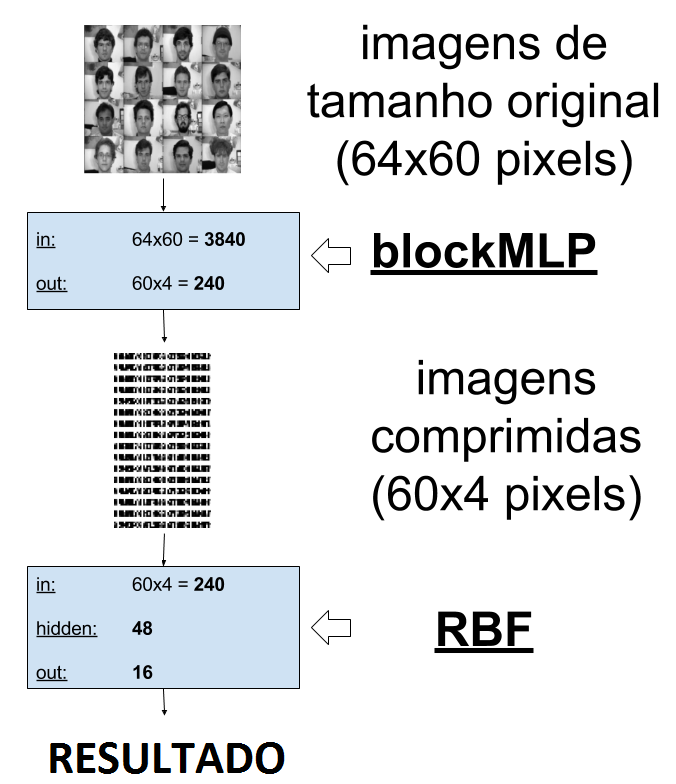
\includegraphics[width = 1\linewidth]{blockmlprbf.png}
\setlength{\abovecaptionskip}{0pt}
\setlength{\belowcaptionskip}{0pt}
\caption{Redes neurais do projeto}
\label{redesdoprojeto}
\end{figure}


\subsection{Entradas e saídas}

Nos blocos azuis da Figura~\ref{redesdoprojeto} vemos o número de entradas e saídas das redes.

Na rede blockMLP, o número de neurônios na camada de entrada é o número total de pixels da imagem original (no exemplo dado, 64x60 pixels = 3840), e o número de neurônios de saída é 240 para ter imagens comprimidas de 60x4.

Já a rede RBF possui 240 neurônios na camada de entrada por esse ser o número de neurônios na saída da compressão da rede blockMLP, e o número de neurônios de saída é o número total de possibilidades de identidades (no exemplo dado, eram 16 pessoas possíveis).

\subsection{Número de camadas escondidas}

Como a rede blockMLP serve simplesmente para a compressão da imagem, ela não possui uma camada escondida (não faz extração de características).

A rede RBF, por sua vez, possui uma camada escondida com 48 neurônios por se tratar de uma rede neural classificadora. Essa camada escondida faz a extração das características necessárias para a identificação das pessoas.

\subsection{Função de ativação}

A função de ativação escolhida foi a função sigmóide, a função de ativação mais comum na construção de redes neurais \cite{haykin}, como pode-se ver na Equação~\ref{eq:sigmoide}:

\begin{equation}
\Phi(v) = \dfrac{1}{1+e^{(-av)}}
\label{eq:sigmoide}
\end{equation}

Enquanto a função de Heavyside (degrau unitário) assume apenas os valores 0 ou 1, a função sigmóide pode assumir todos os valores entre 0 e 1, o que a torna diferenciável. Esse é um ponto importante para o treinamento da rede escolhida.

\subsection{Treinamento da rede}

O algoritmo escolhido para o treinamento da rede é o de retropropagação do erro, descrito pela Equação~\ref{eq:backprop} (para mais informações de como funciona esse tipo de treinamento, consultar Haykin, 1999 \cite{haykin}). 

\begin{equation}
\Delta w_{ji}(n) = \eta \ X \ \delta_{j}(n) \ X \ y_{i}(n)
\label{eq:backprop}
\end{equation}

Onde:

\

$\Delta w_{ji}(n)$ = Correção do peso

$\eta$ = Parâmetro de aprendizado

$\delta_{j}(n)$ = Gradiente local

$y_{i}(n)$ = Sinal de entrada do neurônio anterior

\


Como a totalidade da rede pode ser resumida por uma rede RBF com 3 camadas escondidas, o treinamento se dá da seguinte forma:

\begin{enumerate}
	\item Pelo menos 3 fotos de cada pessoa é colocada na entrada (na entrada da rede blockMLP)
	\item O usuário ensina a rede as respostas esperadas para cada uma das fotos dando a saída correta delas (a saída da rede RBF)
	\item A partir da última camada e até a primeira, os ajustes dos pesos dos neurônios se propagam a cada iteração até que um limiar de sucesso seja atingido
\end{enumerate}

\section{Conclusões}

Este trabalho mostra que é suficientemente simples a construção e treinamento de uma rede neural de reconhecimento facial com uma taxa de sucesso acima de 80\%. 

Se levarmos em conta ainda que o software MATLAB pode ser utilizado para que a implementação da rede e do algoritmo de treinamento não sejam necessários (estes já vêm instalados no software), vemos que qualquer um é capaz de treinar e testar o funcionamento desse tipo de rede neural.

Como sugestão de futuras melhorias, poderia ser feita uma implementação completa dessa rede neural na linguagem C++ para se ter controle total sobre os algoritmos de treinamento, dessa forma podendo medir com mais segurança o desempenho da rede.

Tendo feito esse passo, uma verificação das taxas de sucesso da Tabela~\ref{tab:redes} também teria um valor muito grande.

Concluindo, o potencial para as redes neurais de reconhecimento facial é enorme, haja visto o número de aplicações, e a sua implementação é altamente acessível.

\

%\centering{ \Large{ \textbf{Referências}}}

\begin{thebibliography}{1}
  
  	\bibitem{fagertun} 		FAGERTUN, J. {\em Face Recognition}. 209 f. Dissertação (Mestrado) - Programa de Mestrado em informática e modelagem matemática, Universidade Técnica da Dinamarca, 2005. Disponível em: \url{http://etd.dtu.dk/thesis/185830/imm4014.pdf}. [Acesso em 11 de novembro de 2015].
	
	\bibitem{yesu}	 			YESU, Kolhandai. {\em Hybrid Features Based Face Recognition Method Using Artificial Neural Network}. National Conference on Emerging Trends and Applications in Computer Science, 2012.
	
	\bibitem{nightingale} 	LINGGARD, R.; MYERS, D.J.; NIGHTNGALE, C. {\em Neural Networks for Vision, Speech and Natural Language}. Estados Unidos da América: Springer Science \& Business Media, 2012.
	
	\bibitem{balasuriya} 	BALASURIYA, L. S. {\em Frontal View Human Face Detection and Recognition}. 109 f. Tese (Graduação) - Department of Statistics and Computer Science, University of Colombo, 2000. Disponível em:    \url{http://www.dcs.gla.ac.uk/~sumitha/papers/sumitha_undergraduate_thesis.pdf}. [Acesso em 09 de novembro de 2015].

	\bibitem{le}					LE, Thai Hoang. {\em Applying Artificial Neural Networks for Face Recognition}. Disponível em: \url{http://www.hindawi.com/journals/aans/2011/673016/} [Acesso em 27 de outubro de 2015].

	\bibitem{li}					LI, S. Z. ; JAIN, A. K. {\em Handbook of Face Recognition}. Springer, Nova Iorque, NY, Estados Unidos da América, 2004.

	\bibitem{yale}				Yale Face Database. Disponível em \url{http://vision.ucsd.edu/content/yale-face-database}. [Acesso em 15 de março de 2016].

	\bibitem{viola-jones}	VIOLA, P.; JONES, M. {\em Rapid object detection using a boosted cascade of simple features}. Proceedings of the IEEE Computer Society Conference on Computer Vision and Pattern Recognition, pp. 511–518, dezembro de 2001.
		
	\bibitem{oravec} 			ORAVEC, Miloš; PAVLOVIČOVÁ, Jarmila. {\em Face Recognition Methods Based on Feedforward Neural Networks, Principal Component Analysis and Self-Organizing Map}.Radioengineering, vol.16, no.1, Bratislava, Eslováquia, Abril de 2007.
	
	\bibitem{haykin}			HAYKIN, Simon. {\em Neural networks and learning machines}.3 ed. Estados Unidos da América: Pearson, 1999.

  \end{thebibliography}

\end{document}

%\begin{figure}[H]
%\centering
%\begin{minipage}[b]{0.45\linewidth}
%\centering
%\graphicspath{{Imagens/}}
%
\includegraphics[width = 0.7\linewidth]{UTFPR.png}
%\setlength{\abovecaptionskip}{0pt}
%\setlength{\belowcaptionskip}{0pt}
%\caption{Figure obtenue sur la caméra en ne laissant passer que l'ordre 0}
%\label{fig:minipage1}
%\end{minipage}
%\quad
%\begin{minipage}[b]{0.45\linewidth}
%\centering
%\graphicspath{{Imagens/}}
%
\includegraphics[width = 0.7\linewidth]{UTFPR.png}
%\setlength{\abovecaptionskip}{0pt}
%\setlength{\belowcaptionskip}{0pt}
%\caption{Figure obtenue sur la caméra en masquant l'ordre 0}
%\label{fig:minipage2}
%\end{minipage}
%\end{figure}

%\begin{table}[H]
%\centering
%\begin{tabular}{|c|c|c|c|}
%\hline
%Matheus & Tabela & super & legal \\ \hline
%1 & 2 & 3 & 4 \\ \hline
%\end{tabular}
%\title{My first table}
%\label{tab:minha_tabela}
%\end{table}